\documentclass{beamer}
\usetheme{Boadilla}
\usepackage[utf8]{inputenc}
\usepackage{appendixnumberbeamer}
\setbeamercolor{alerted text}{fg=red!150!black!100}  %
%\usecolortheme{fly} \setbeamercolor{alerted text}{fg=white}  %
%\usecolortheme{seagull}
%\usecolortheme{dove}

\usepackage[normalem]{ulem}
\newcommand\aN{^{N}}

\newcommand\gagnerduTemps[1]{#1}
%\newcommand\gagnerduTemps[1]{}

\definecolor{green}{rgb}{0.0, 0.6, 0.0}
\definecolor{red}{rgb}{0.7, 0.0, 0.0}
\definecolor{blue}{rgb}{0.0, 0.0, 0.8}

\beamertemplatenavigationsymbolsempty
\usepackage{tikz}
\usepackage{appendixnumberbeamer}
\usetikzlibrary{shapes,arrows,positioning,automata}
\everymath{\displaystyle}

\newcommand\mpage[2]{%
  \begin{minipage}{#1\linewidth}%
    #2%
  \end{minipage}%
}

%%%%%%%%%%%%%%%%%%%%%%%%%%%%%%%%%%%%%%%%%%%%%%%%%%%%%%%%%%%%%%%%%%%%%%%%
%%% The following black magic puts copies of the table of contents
%%% throughout your talk: you might not want this.
\AtBeginSection[]
{
  \begin{frame}{Outline}
    \tableofcontents[current,currentsection]
  \end{frame}
}
%%%%%%%%%%%%%%%%%%%%%%%%%%%%%%%%%%%%%%%%%%%%%%%%%%%%%%%%%%%%%%%%%%%%%%%%


\newcommand\dt{\frac{d}{dt}}
\newcommand\esp[1]{\mathbb{E}\left[#1\right]}
\newcommand\var[1]{\mathrm{var}\left[#1\right]}
\graphicspath{{../simu/output_pdfs/}{}{figs/}}

\definecolor{violet}{rgb}{0.3, 0., 0.2}
\definecolor{darkgreen}{rgb}{0, 0.2, 0}
\setbeamercolor{math text}{fg=violet}
\newcommand\red[1]{{\color{red}#1}}
\newcommand\blue[1]{{\color{blue}#1}}
\newcommand\green[1]{{\color{green}#1}}
\newcommand\bx{\mathbf{x}}


\newcommand\bm{\mathbf{m}}
\newcommand\expect[1]{\mathbb{E}\left[#1\right]}
\newcommand\E{\mathbb{E}}
\newcommand\p[1]{\left(#1\right)}
\newcommand\calS{\mathcal{S}}
\newcommand\calE{\mathcal{E}}
\newcommand\calA{\mathcal{A}}
\newcommand\calB{\mathcal{B}}
\newcommand\calT{\mathcal{T}}
\newcommand\calP{\mathcal{P}}
\newcommand\calL{\mathcal{L}}
\newcommand\Proba[1]{\mathbf{P}\left[#1\right]}
\newcommand\proba[1]{\mathbf{P}\left[#1\right]}
\newcommand\norm[1]{\left\|#1\right\|}
\newcommand\abs[1]{\left|#1\right|}
\newcommand\N{\mathbb{Z}^+}
\newcommand\R{\mathbb{R}}
\newcommand\bbm{\mathbf{m}}
\newcommand\bX{\mathbf{X}}
\newcommand\bE{\mathbf{E}}
\newcommand\LN{L^{(N)}}
\newcommand\bl{{\text{\boldmath$\ell$}}}

\DeclareMathOperator*{\argmin}{arg\,min}

\setbeamertemplate{blocks}[rounded][shadow=false]
\setbeamercolor*{block title}{fg=blue!70!black!90, bg=blue!8}
\setbeamercolor*{block body}{bg=blue!4}

\tikzset{every picture/.append style={shorten >=2pt,line width=2pt}}
\tikzstyle{wide}=[line width=2pt,->]

\makeatother
\setbeamertemplate{footline}
{
  \hfill 
  \usebeamerfont{author in head/foot}\insertshortauthor{} -- 
  \insertframenumber{} / \inserttotalframenumber\hspace*{1ex}
  \vskip0pt%
}
\makeatletter

\begin{document}

\title{A Refined Mean Field Approximation\\ for Synchronous Population
  Processes}%
% \subtitle{Beyond mean field models}%
\author{Nicolas Gast}%
\institute{Inria, Grenoble, France (joint work with Diego Latella and
  Mieke Massink, CNR/ISTI (Italy))}%
\date{MAMA Workshop, 2018}%

\maketitle


% \begin{frame}{Good system design needs performance evaluation}
%   {In this talk : stochastic model}
%   %$N$ objects. \bigskip

%   \begin{tikzpicture}
%     %\node at (0,0) {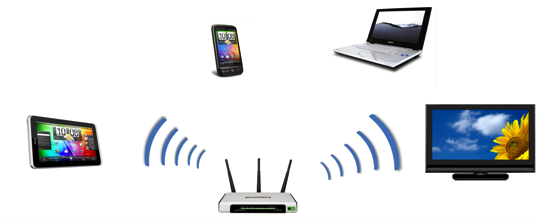
\includegraphics[width=.5\linewidth]{wifi}};
%     %\node at (-1,1) {Wifi: object = device}; 
%     %\node at (6,-2) {\includegraphics[width=.4\linewidth]{cache}};
%     %\node at (7.5,-3) {object = content}; 
%     \node at (0,-4.5) {
\includegraphics[width=.4\linewidth]{cluster-server}};
%     %\node at (0,-6.5) {Cluster: object = server};

%     %\uncover<2>{
%     \node at (6,-5) {\includegraphics[width=.3\linewidth]{perf_xkcd}};
%     \node at (6.4,-4.75) {\Huge \textbf{???}};
%     %}
%   \end{tikzpicture}
% \end{frame}


\begin{frame}{How to characterize emerging behavior starting from a
    stochastic model of interacting objects? }
  %$N$ objects. \bigskip

  \begin{tikzpicture}
    \node at (0,0) {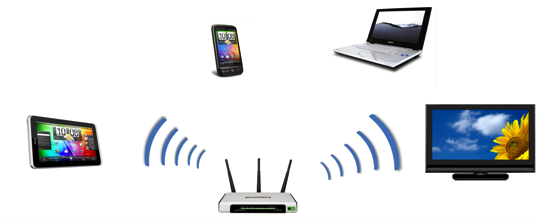
\includegraphics[width=.5\linewidth]{wifi}}; \node
    at (-2,-1) {Wireless}; %
    \node at (6,-2.5) {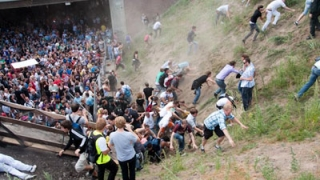
\includegraphics[width=.4\linewidth]{foule}};
    \node at (7.5,-4) {Evacuation}; %
    \node at (0,-4.5)
    {
\includegraphics[width=.4\linewidth]{cluster-server}}; \node at
    (-2,-3.5) {Cloud};
  \end{tikzpicture}
\end{frame}


\begin{frame}{Thanks to the law of large numbers : Some systems
    simplify as they grow}

  \begin{align*}
    % "\text{\color{blue}Theorem}". \qquad
    \lim_{N\to\infty}\left(\begin{array}{c}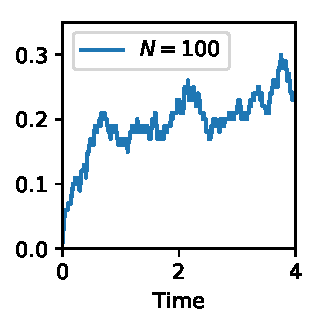
\includegraphics[width=.28\linewidth]{traj_rho80_onlyN100}\end{array}\right) 
    =\underbrace{\begin{array}{c}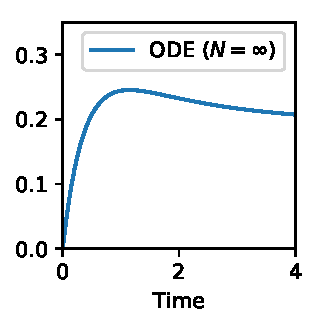
\includegraphics[width=.28\linewidth]{traj_rho80_onlyNinf}\end{array}}_{
    \text{Mean field approximation}}
  \end{align*}
  
  
  Applications : 
  \begin{itemize}
  \item Communication protocols (MPTCP, Simgrid) 
  \item Mean field games (Adversarial classification)
  \item Performance of load balancing / caching algorithms
  \item Stochastic approximation / learning 
  \item Theoretical biology 
  \end{itemize}
\end{frame}

\newcommand\marque[2]{\draw (#1,-0.2) -- (#1,0.2);\node at (#1,.5){$N=#2$};}

% \begin{frame}{What happened is a law of large numbers}
%   {Some systems simplify as $N$ goes to infinity : objects become independent}
%   % (\emph{a.k.a.} mean
%   % field approximation)}
%   \begin{align*}
%     "\text{\color{blue}Theorem}". \qquad\lim_{N\to\infty}\left(\begin{array}{c}\includegraphics[width=.28\linewidth]{traj_rho80_onlyN1000}\end{array}\right) 
%     =\underbrace{\begin{array}{c}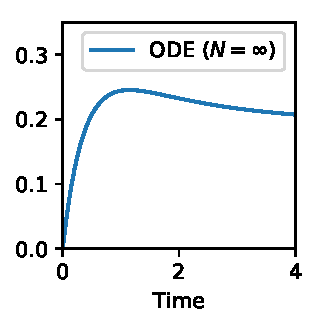
\includegraphics[width=.28\linewidth]{traj_rho80_onlyNinf}\end{array}}_{
%     \text{Mean field approximation}}
%   \end{align*}

  
%   Mean field approximation has been shown to be asymptotically exact
%   and has been successfully used in many context. For example : 
%   \begin{itemize}
%   \item CSMA (see \emph{e.g.} Thesis of F. Cecchi), 802.11 (Bianchi's
%     formula)
%   \item Load balancing (power of two-choice, Mitzenmacher 98 /
%     Vvedenskaya 96, Tsitsiklis,Xu 2011\& 2013)
%   \item Caching algorithms (G and Van Houdt 2015)
%   \end{itemize}

  
% \end{frame}

\begin{frame}{We can study large systems. What about moderate sizes?} 
  
  \begin{tikzpicture}
    \draw[->] (0,0) -- (11,0);
    % \draw[color=darkgreen,dashed] (0.5,-.2) -- (0.5,1.5);
    % \node[color=green,draw,fill=white] at (0.5,1.5){$N=1$: easy};
    \draw[color=darkgreen,dashed] (10.5,-.2) -- (10.5,1.5);
    \node[color=green,draw,fill=white] at (10.5,1.5){$N=\infty$: easy};

    \uncover<1->{
      % \marque{1}{1};
      \marque{2}{10};%
      \marque{5}{100};%
      \marque{8}{1000};%
      \draw[color=red!50,fill,opacity=.2] (1,-1) rectangle (9,1.5); 
      \node[red] at (5,1){What can we do here?};
    }
    % \marque{11}{1000};
    
    \uncover<2->{
      \node[darkgreen,draw] at (5,-3) (P) {\mpage{.45}{For many
          systems, asymptotically: 
          
          \centering
          $\displaystyle Perf(N) \approx Perf(\infty) + \frac1N V $
        }}; %
      % \draw[darkgreen,->] (5,-1) -- node[right] {purpose of this talk}
      % (P);

    }
    \uncover<3->{
      \node at (4,-4.5) (MF) {Mean field approximation}; 
      \node at (6,-5.5) (RMF) {\emph{Refined} mean field approximation}; 
      \draw[->,line width=1pt] (5,-3.3) -- (MF);
      \draw[dashed,line width=1pt] (4.5,-3.55) rectangle (7.25,-2.75); 
      \draw[->,line width=1pt] (6,-3.55) -- (RMF);
    }
    
  \end{tikzpicture}
\end{frame}


\begin{frame}{Outline}
  \tableofcontents
\end{frame}



\section{Mean field approximations of synchronous populations}

\begin{frame}{Discrete-time mean field models}
  Population of $N$ objects (discrete time, discrete space).
  \begin{align*}
    X_i(t) = \text{fraction of object in state $i$ at time $t$}
  \end{align*}

  \pause \vspace{1cm}%
  There are two cases:
  \begin{itemize}
  \item \blue{Asynchronous case} (BLB08,K81) -- One (or a few) objects
    change state at each time step. {\small(see talk at
      SIGMETRICS)}
    \begin{itemize}
    \item \red{Continuous-time} mean field approximation
    \end{itemize}
    \bigskip
    
  \item \blue{Synchronous case} (LB+07) -- All object simultaneously
    change state {\small (\blue{this talk})}.
    \begin{itemize}
    \item \red{Discrete-time} mean field approximation
    \end{itemize}
  \end{itemize}

  \vspace{1.5cm}{
    \tiny
    \begin{itemize}
    \item[BLB08] Michel Benaïm, Jean-Yves Le Boudec: A class of mean
      field interaction models for computer and communication
      systems. Perform. Eval. 2008
    \item[K81] Thomas G. Kurtz : Approximation of Population
      Processes. 1981
    \item[LB+07] Jean-Yves Le Boudec, David D. McDonald, Jochen
      Mundinger: A Generic Mean Field Convergence Result for Systems
      of Interacting Objects. QEST 2007
    \end{itemize}
  }
\end{frame}

\begin{frame}{Our synchronous model is similar to the one of [LB+07]}
  
  At each time step : all objects perform an independent transition :
  \begin{align*}
    K_{ij}(x) = \Proba{\text{An object in state $i$
    changes to state $j$} \mid X(t)=x}.
  \end{align*}
  
  The mean field approximation is given by :
  \begin{align*}
    \mu(t+1) = \mu(t)K(\mu(t)) \blue{=: \Phi_1(\mu(t))}
  \end{align*}

  \bigskip The mean field approximation is asymptotically exact
  (LB+07) :
  \begin{align*}
    X(t)=\mu(t)+o_{N\to\infty}(1).
  \end{align*}
\end{frame}

\begin{frame}{Example : a simple infection model (SEIR model)}

  \mpage{.4}{
  Evolution of one individual:}
  \mpage{.5}{
    \begin{tikzpicture}
      \tikzstyle{state}=[circle,draw]
      \node[state] at (0,0) (S) {S};
      \node[state] at (4,0) (E) {E};
      \node[state] at (4,-2) (I) {I};
      \node[state] at (0,-2) (R) {R};
      \draw(S) edge[->] node[above]{$\alpha_E+\alpha_I \blue{X_I}$} (E);
      \draw(E) edge[->] node[left]{$\alpha_A$} (I);
      \draw(I) edge[->] node[above]{$\alpha_R$} (R);
      \draw(R) edge[->] node[right]{$\alpha_L$} (S);
    \end{tikzpicture}
  }\vspace{1cm}\pause

  We plot $\esp{X_S(t)}$ as a function of time :
  \begin{tabular}{@{}c@{}c}
    \mpage{.5}{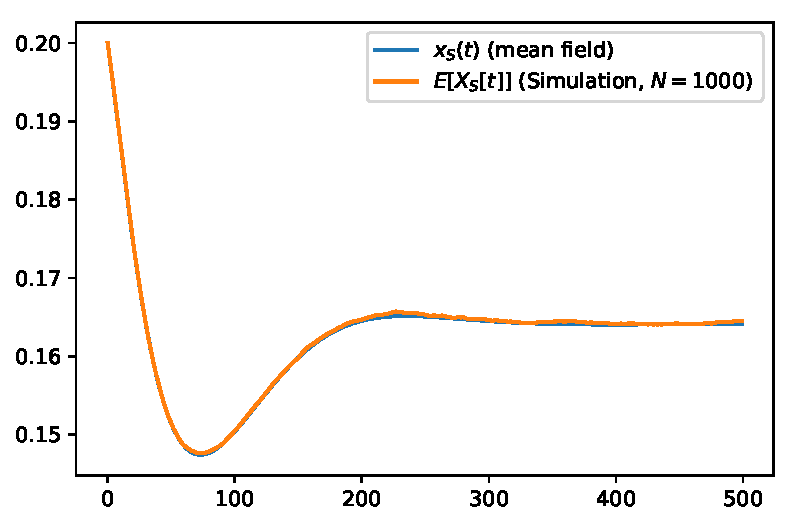
\includegraphics[width=\linewidth]{SEIR_onlyMF_N1000}}
    &\uncover<3->{\mpage{.5}{%
      \only<1-3>{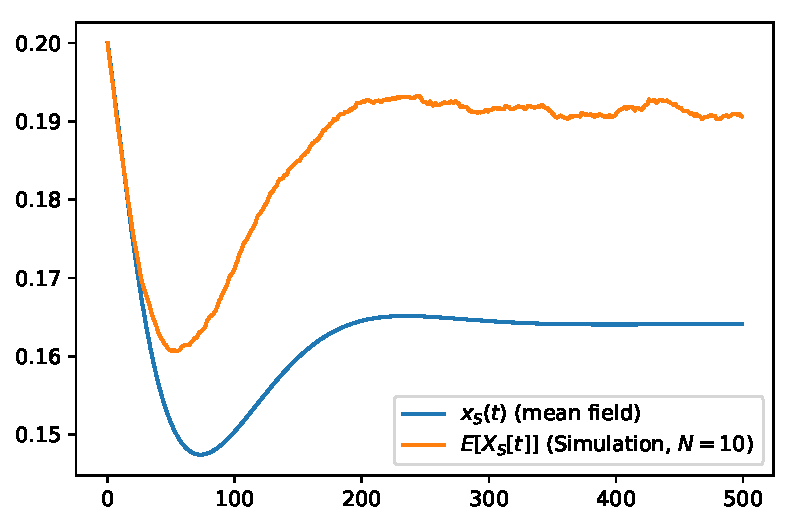
\includegraphics[width=\linewidth]{SEIR_onlyMF_N10}}
      \only<4->{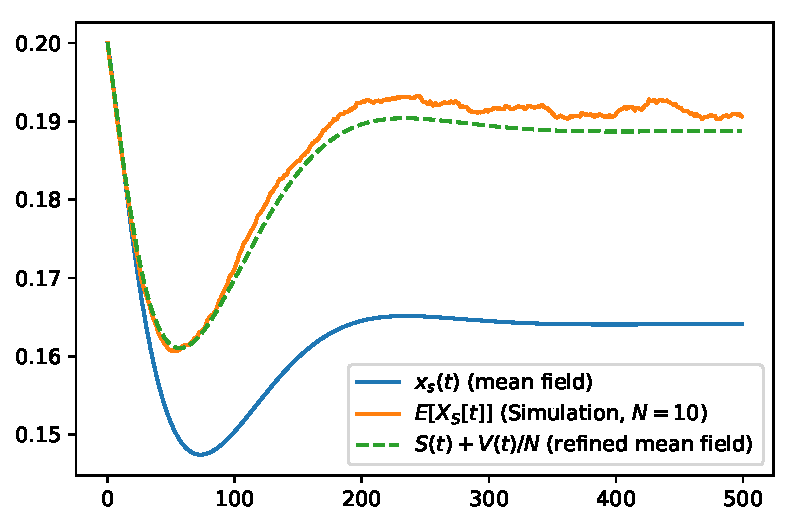
\includegraphics[width=\linewidth]{SEIR_all_N10}}}
      }\\
    $N=1000$ & \uncover<3->{$N=10$}
  \end{tabular}
\end{frame}

\section{The refined mean field}

\begin{frame}{First result : transient regime}

  We assume that $\Phi_1:x\mapsto xK(x)$ is twice differentiable and 
  we define
    \begin{align*}
      A(t)=(D \Phi_1)(\mu(t)) \text{ and } B(t) = (D^2 \Phi_1)(\mu(t))\\
      \begin{array}{rl}
        \Gamma_{jk}({x}) & = \sum_{i=1}^n x_i
                           {K}_{ij}({x})\p{\mathbf{1}_{j=k}-{K}_{ik}({x})} 
      \end{array}
    \end{align*}

    Let$V(0)=0$, $W(0) = 0$ and
    \begin{align}
      \begin{array}{rl}
        V(t+1) & = A(t)V(t) + \frac{1}{2}B(t) \cdot W(t)\\
        W(t+1) & = \Gamma(\mu(t)) + A(t) W(t) A(t)^T.
      \end{array}
                  \label{eq:VW}
    \end{align}
    \begin{theorem}[Transient Regime]\label{theo:main}
      For any time $t$ :
      $\esp{X(t)}= \mu(t) + \frac1N V(t) + o(1/N)$.
    \end{theorem}
\end{frame}

\begin{frame}{Second result : steady-state}

  We assume that in addition, the mean field approximation has a
  unique fixed point that is exponentially stable :
  $\abs{\Phi_t(m)-\pi}\le ae^{-bt}$. 
  
  \pause 
  \begin{theorem}
    If the mean field approximation has a unique exponentially stable
    fixed point, then the previous theorem holds \emph{uniformly in
      time}.

    In particular in steady state:
    $\esp{X}= \pi + \frac1N\p{\lim_{t\to\infty}V(t)} + o(1/N)$.
  \end{theorem}

  \only<1-3>{
    \begin{center}
      \mpage{.9}{%
        \begin{tikzpicture}
          \node at
          (0,0){%
            \only<1-2>{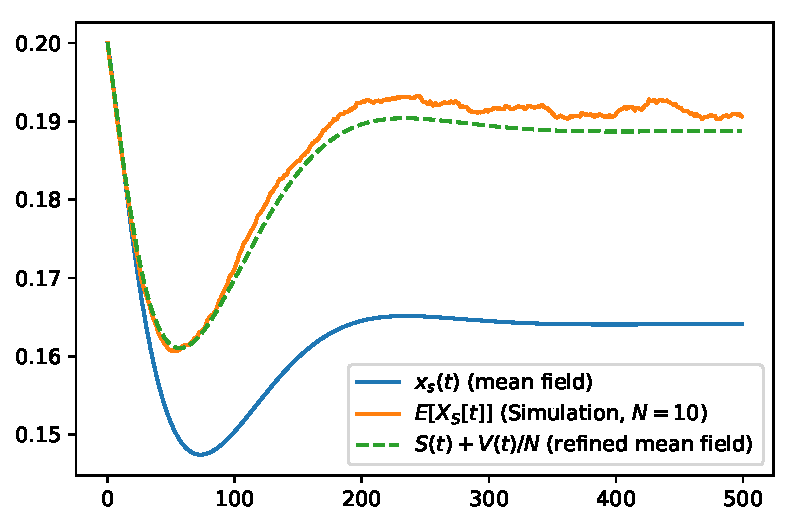
\includegraphics[width=.7\linewidth]{SEIR_all_N10}}%
            \only<3->{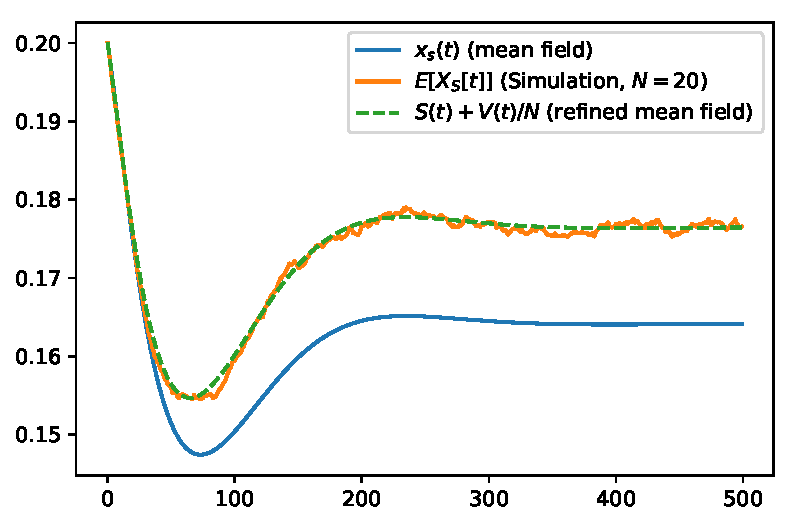
\includegraphics[width=.7\linewidth]{SEIR_all_N20}}};
          \only<1-2>{\node at (5.5,1.5){Refined m.f. $\mu(t)+\frac{V_t}{10}$};}
          \only<3>{\node at (5.5,0.5){Refined m.f. $\mu(t)+\frac{V_t}{20}$};}
          \node at (5,-.5){Mean field $\mu(t)$};
        \end{tikzpicture}
      }
    \end{center}
  }
  \only<4>{
    \blue{Result for steady-state:}
    
    \begin{tabular}{@{}|c|ccccc|c|}
      \hline
      &$N$&$10$&$20$&$30$&$50$&$\infty$ (mf)\\\hline
      $\esp{X_S}$ (Simulation)&0.191 & 0.177 & 0.175 & 0.169 & 0.166 & --\\
      $\mu_S(\infty)+\frac{V}{N}$ (Refined mf)&0.189 & 0.176 & 0.172 & 0.169 & 0.167 & 0.164\\\hline
    \end{tabular}
    }
\end{frame}

\begin{frame}{Where does the $O(1/N)$-term come from?}
  The mean field approximation is $\mu(t{+}1){=}\mu(t)K(\mu(t))$ with
  $\mu(0){=}M(0)$. 
  \begin{align*}
    \esp{X(t+1)\mid X(t)=\mu(t)} &= \mu(t) K(\mu(t)) = \mu(t+1)
  \end{align*}
  Hence :
  \begin{align*}
    \esp{X(t+1)} &= \esp{X(t) K(X(t))}
                   \uncover<2->{\blue{\text{\only<3>{\sout}{$\approx\esp{X(t)} K(\esp{X(t)})$}}}%
                   &\blue{\text{Mean field approx.}}}
  \end{align*} \pause \pause
  
  Now, in addition :
  \begin{align*}
    \mathrm{cov}(X(t),X(t) \mid X(t)=\mu(t)) &\blue{=
                                               \frac1N\Gamma(\mu(t))}. 
  \end{align*}
  The refined mean field is derived by taking the $1/N$-term into
  account.
\end{frame}


   
\section{Does it always work?}

\begin{frame}{Positive side}

  Many models satisfy the assumptions (see paper).
  \begin{itemize}
  \item Refined model is easy to compute (linear algebra)
  \item It improves the accuracy for not so large values of $N$.
  \end{itemize}
\end{frame}

\begin{frame}{Limit of the approach on an example}
  \begin{columns}
    \begin{column}{.4\linewidth}
      \begin{tikzpicture}
        \tikzstyle{state}=[circle,draw]
        \node[state] at (0,0) (0) {0};
        \node[state] at (3,0) (1) {1};
        \draw (0) edge[bend left,->] node[above] {$\alpha x_0$} (1);
        \draw (1) edge[bend left,->] node[above] {$1$} (0);
      \end{tikzpicture}
    \end{column}
    \begin{column}{0.4\linewidth}
      \centering
      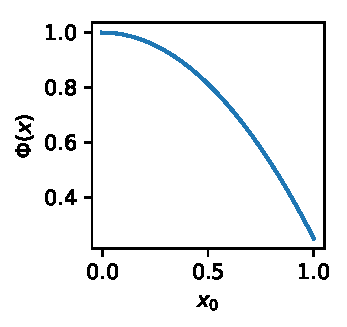
\includegraphics[width=.8\linewidth]{phi_unstable}
      \vspace{-1cm}
      
      \begin{align*}
        \Phi_1(x_0) &= 1-\alpha (x_0)^2
      \end{align*}
    \end{column}
  \end{columns}
  \bigskip\bigskip
  
  \begin{itemize}
  \item There is a unique fixed point $\pi$. 
  \item It is an attractor \emph{iff} $\alpha\le0.75$. 
  \item It is exponentially stable \emph{iff} $\alpha<0.75$. 
  \end{itemize}
\end{frame}

\begin{frame}{Example (continued) : numerical illustration}
  % \begin{tikzpicture}
  %   \node at (0,0) {\mpage{1}{
  \begin{tikzpicture}
    \only<1>{%
      \node at (0,0) {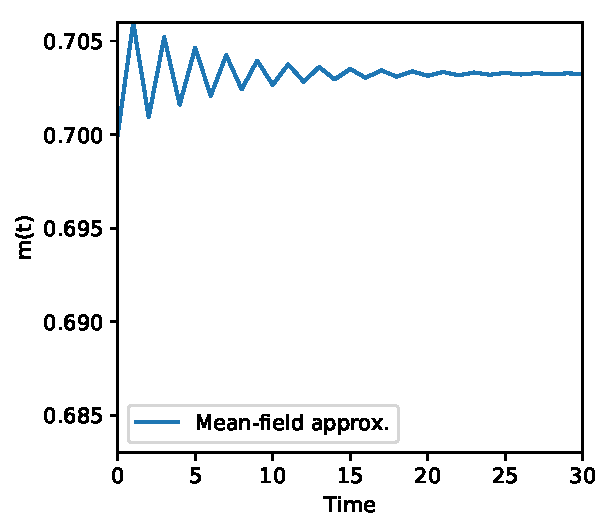
\includegraphics[width=.45\linewidth]{unstable1D_onlyMFa60_N10}};
      \node at (6,0)
      {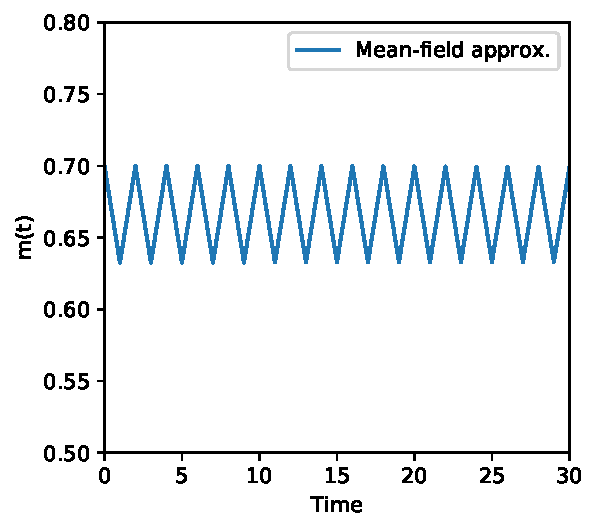
\includegraphics[width=.45\linewidth]{unstable1D_onlyMFa75_N10}};
    }
    \only<2>{%
      \node at (0,0) {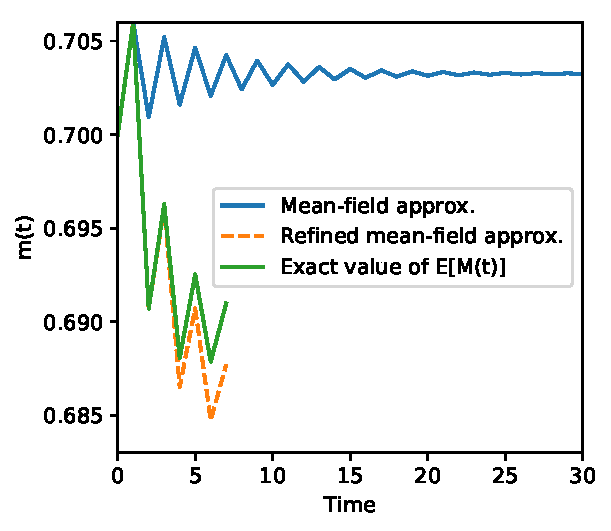
\includegraphics[width=.45\linewidth]{unstable1D_TL_a60_N10}};
      \node at (6,0)
      {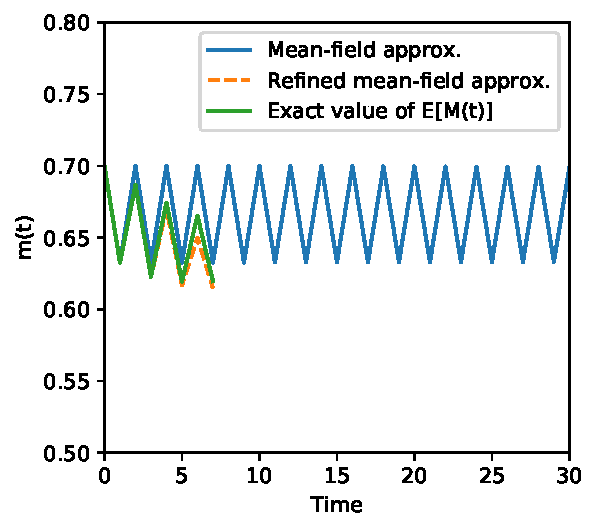
\includegraphics[width=.45\linewidth]{unstable1D_TL_a75_N10}};
    }
    \only<3>{%
      \node at (0,0) {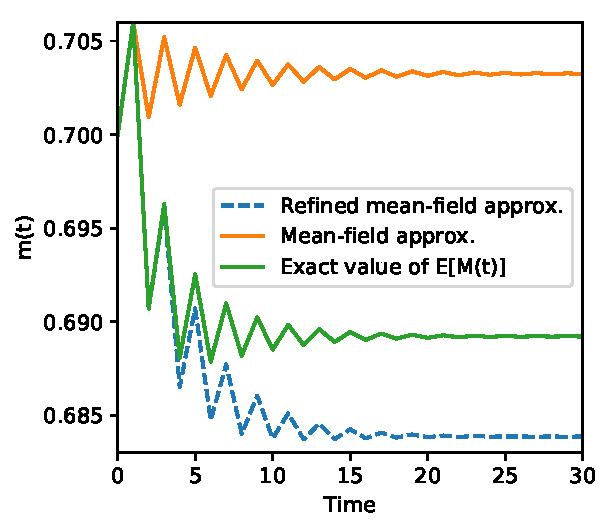
\includegraphics[width=.45\linewidth]{unstable1D_a60_N10}};
      \node at (6,0)
      {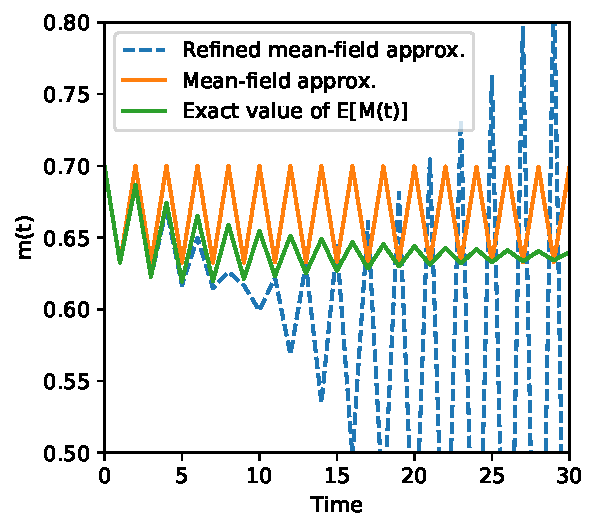
\includegraphics[width=.45\linewidth]{unstable1D_a75_N10}};
    }
    \only<4>{%
      \node at (0,0) {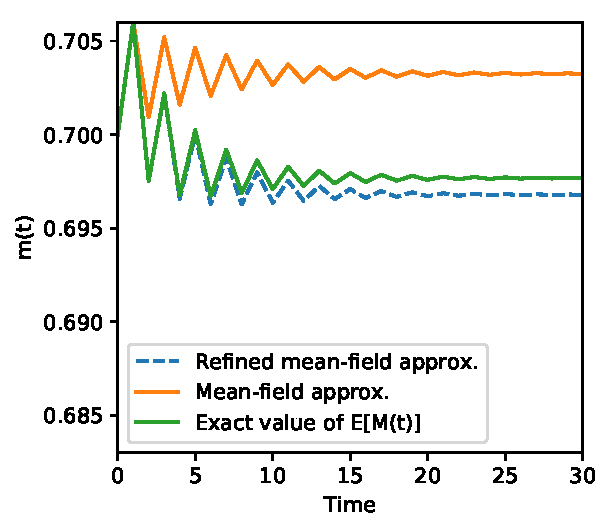
\includegraphics[width=.45\linewidth]{unstable1D_a60_N30}};
      \node at (6,0)
      {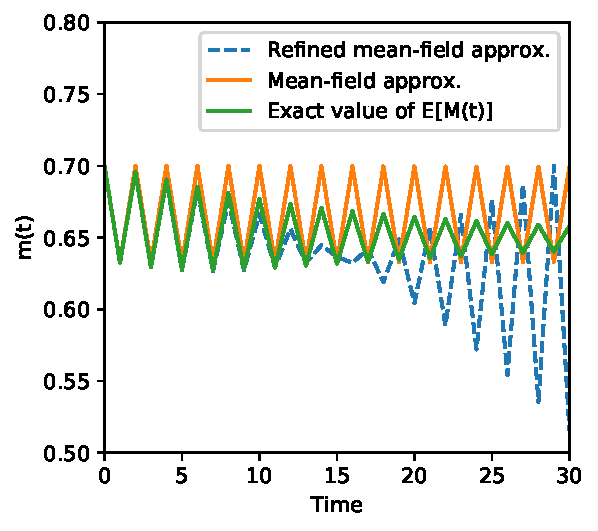
\includegraphics[width=.45\linewidth]{unstable1D_a75_N30}};
    }

    \only<1-3>{\node[fill=white] at (3,-2) {\Large $N=10$};}
    \only<4->{\node[fill=white] at (3,-2) {\Large $N=30$};}
    
    % \only<2>{\mpage{.45}{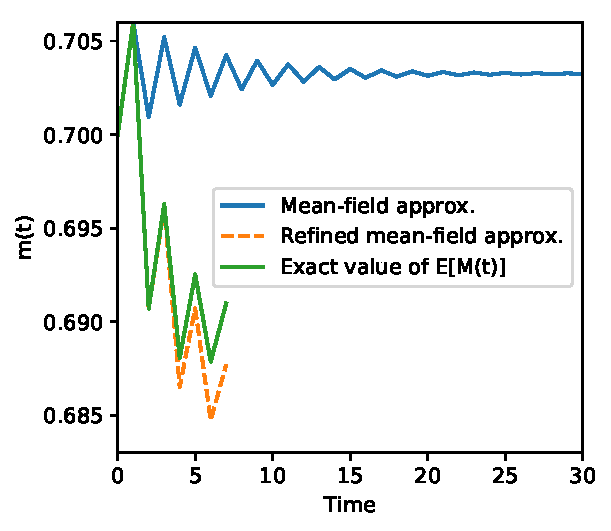
\includegraphics[width=\linewidth]{unstable1D_TL_a60_N10}}}%
    % \only<3>{\mpage{.45}{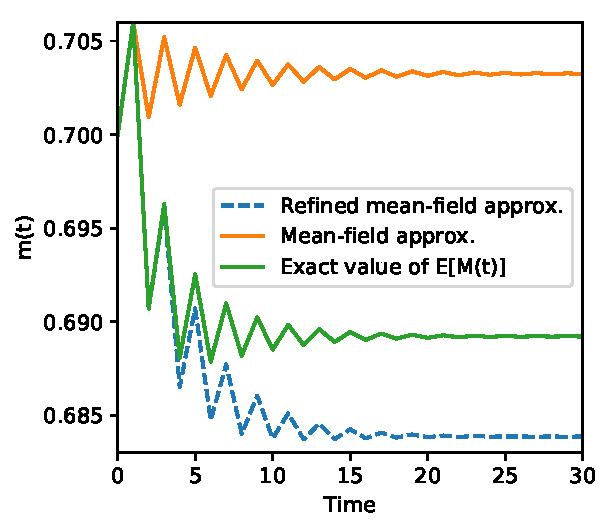
\includegraphics[width=\linewidth]{unstable1D_a60_N10}}}%
    % \only<4>{\mpage{.45}{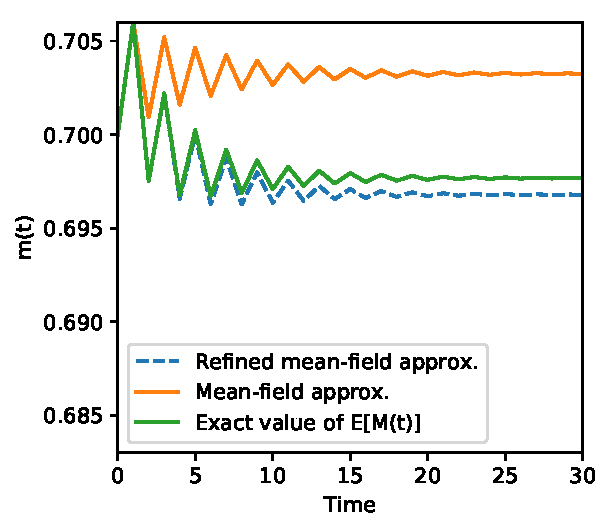
\includegraphics[width=\linewidth]{unstable1D_a60_N30}}}
    % %
    % \only<1>{\mpage{.45}{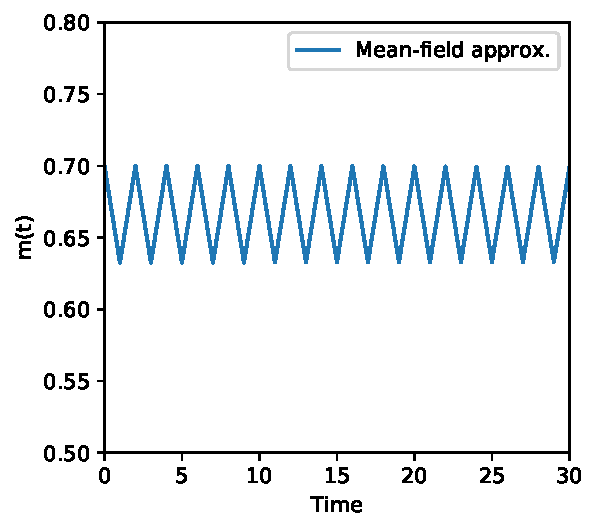
\includegraphics[width=\linewidth]{unstable1D_onlyMFa75_N10}}}%
    % \only<2>{\mpage{.45}{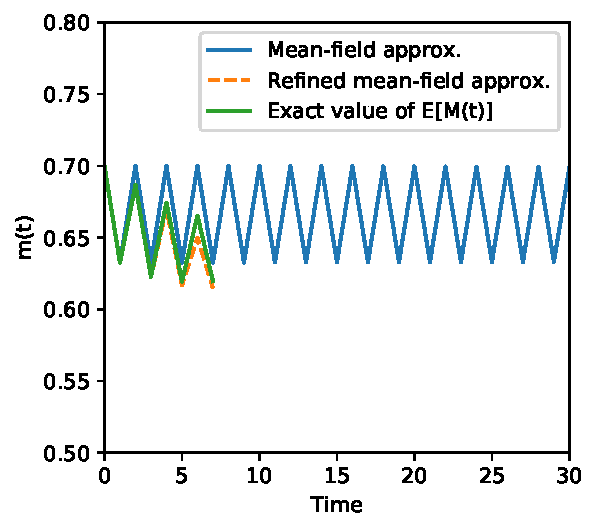
\includegraphics[width=\linewidth]{unstable1D_TL_a75_N10}}}%
    % \only<3>{\mpage{.45}{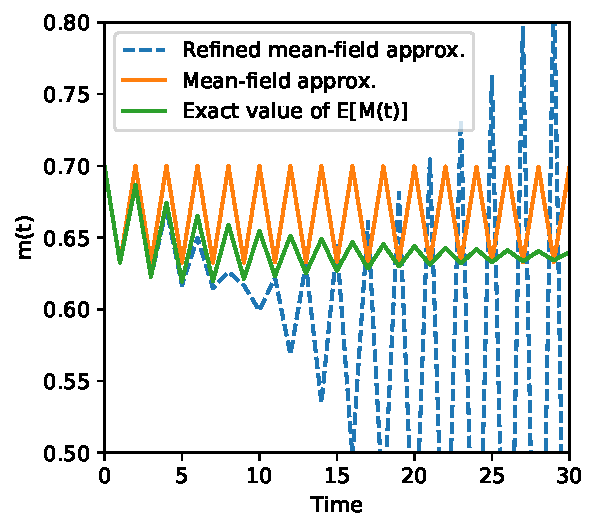
\includegraphics[width=\linewidth]{unstable1D_a75_N10}}}%
    % \only<4>{\mpage{.45}{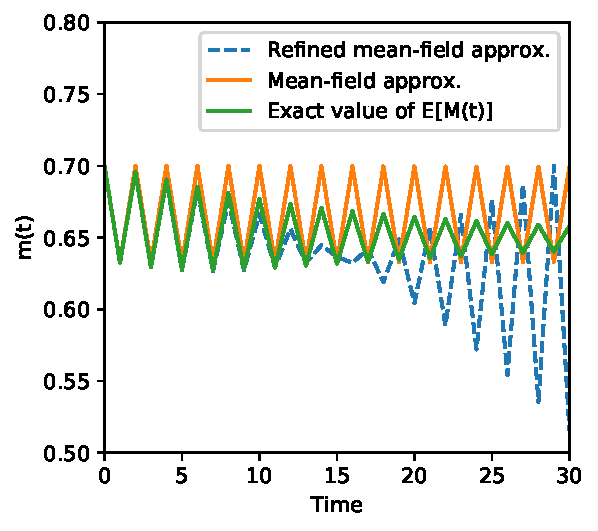
\includegraphics[width=\linewidth]{unstable1D_a75_N30}}}%
  \end{tikzpicture}

    
      \begin{tabular}{cc}
        \mpage{.45}{~}&\mpage{.45}{~}\\
      $a=0.6$ (exponentially stable) & $a=0.75$ (not exp. stable). \\
      ~\\\pause\pause
      \textbf{WORKS uniformly in $t$}&\textbf{Does not work for $t\gg N$}
    \end{tabular}
    % };
    % }
    % \end{tikzpicture}
                                       \end{frame}

\section{Conclusion and recap}

\begin{frame}{Recap}
  
  \begin{enumerate}
  \item The traditional mean field approximation considers
    \begin{align*}
      X(t) \approx \mu(t),
    \end{align*}
    where $\mu(t) = \lim_{N\to\infty}X(t)$. 
    
  \item Our approach : we focus on $\esp{X(t)}$ and we show that there
    exists $V(t)$ such that :
    \begin{align*}
      \esp{X(t)} = \underbrace{\mu(t) + \frac{V(t)}{N}}_{\blue{\text{Refined
      approximation}}} + o(1/N) 
    \end{align*}
    It also works for $\esp{h(X(t))}$. 
  \item $V(t)$ is easy to evaluate and for small $N$ the refined
    approximation greatly improves the accuracy compared to the
    classical mean field approximation.
  \end{enumerate}
\end{frame}

\begin{frame}{To go further : }
  
  It also works for continuous time models (\emph{e.g.}: two-choice),
  see SIGMETRICS paper. \bigskip

  Future work:
  \begin{itemize}
  \item Find a relevant model (more general?) of synchronous
    population.
    % \item Mean field models with multiple equilibria and/or cycles. 
    % \item Can we go to the order $O(1/N^2)$? It is useful?
  \item Find guidelines where the method is applicable or not (example
    : Non-exponentially stable systems)
  \end{itemize}
  
  \bigskip
  
  Main references :
  \begin{itemize}
  \item \blue{A Refined Mean Field Approximation of Synchronous
      Discrete-Time Population Models} by Gast, Latella and
    Massink. To appear in \emph{Performance Evaluation}.
    
    Paper is reproducible :
    \url{https://github.com/ngast/RefinedMeanField_SynchronousPopulation}
  \item \blue{A Refined Mean Field Approximation} by Gast and Van
    Houdt. To appear in SIGMETRICS 2018 {\small
      \url{https://hal.inria.fr/hal-01622054/}}
    \url{https://github.com/ngast/rmf_tool/}
  \end{itemize}
\end{frame}

\end{document}

\appendix

\newcommand\reference[4]{\item[\mpage{.2}{\tiny #1}] \footnotesize 
  \emph{#2}, \tiny #3,  #4}
\begin{frame}{Thank you!}

  %Slides are online at
  \begin{center}
    \url{http://mescal.imag.fr/membres/nicolas.gast}\\ \bigskip
    \texttt{nicolas.gast@inria.fr}
  \end{center}
  \bigskip\bigskip
  
  \qquad\qquad\mpage{.85}{
    Mean field and decoupling
    \begin{itemize}
      \reference{Bena\"im, \\Le Boudec 08}{A class of mean field
        interaction models for computer and communication
        systems}{M.Bena\"im and J.Y. Le Boudec.}{Performance
        evaluation, 2008.}%
      \reference{Le Boudec 10}{The stationary behaviour of fluid
        limits of reversible processes is concentrated on stationary
        points.}{J.-Y. L. Boudec. }{Arxiv:1009.5021, 2010}%
      \reference{Darling Norris 08}{R. W. R. Darling and
        J. R. Norris}{Differential equation approximations for Markov
        chains}{Probability Surveys 2008} %
      % \reference{Kurtz 70}{}{}{}
      \reference{G. 16}{Construction of Lyapunov functions via
        relative entropy with application to caching}{Gast, N.}{ACM
        MAMA 2016}%
      \reference{G. 16}{mean field approximation is $1/N$
        accurate}{Gast, N.}{submitted}%
      \reference{Budhiraja et al. 15}{Limits of relative entropies
        associated with weakly interacting particle
        systems.}{A. S. Budhiraja, P. Dupuis, M. Fischer, and
        K. Ramanan. }{Electronic journal of probability, 20, 2015.}
    \end{itemize}
  }
\end{frame}

\begin{frame}{References (continued)}
  \qquad\qquad\mpage{.85} {
    Optimal control and mean field games: 
    \begin{itemize}
      \reference{G.,Gaujal Le Boudec 12}{Mean field for Markov
        decision processes: from discrete to continuous
        optimization}{N.Gast,B.Gaujal,J.Y.Le Boudec}{IEEE TAC, 2012 }%
      \reference{G. Gaujal 12}{Markov chains with discontinuous drifts
        have differential inclusion limits.}{Gast N. and Gaujal
        B.}{Performance Evaluation, 2012} %
      % \reference{Puterman}{Markov decision processes: discrete
      %   stochastic dynamic programming}{M.L. Puterman}{John Wiley \&
      %   Sons, 2014.} %
      \reference{Lasry Lions}{Mean field games}{J.-M. Lasry and
        P.-L. Lions}{Japanese Journal of Mathematics, 2007.} %
      \reference{Tembine at al 09}{Mean field asymptotics of markov
        decision evolutionary games and teams}{H. Tembine,
        J.-Y. L. Boudec, R. El-Azouzi, and E. Altman.}{GameNets 00}%
    \end{itemize}
    Applications: caches %, bikes 

    \begin{itemize}
      \reference{Don and Towsley}{An approximate analysis of the LRU
        and FIFO buffer replacement schemes}{A. Dan and
        D. Towsley.}{SIGMETRICS 1990}
      \reference{G. Van Houdt 15}{Transient and Steady-state Regime
        of a Family of List-based Cache Replacement Algorithms.}{Gast,
        Van Houdt.}{ACM Sigmetrics 2015}
      % \reference{Fricker-Gast 14}{Incentives and redistribution in
      %   homogeneous bike-sharing systems with stations of finite
      %   capacity.}{C. Fricker and N. Gast. }{ EJTL, 2014.}
      % \reference{Fricket et al. 13}{Mean field analysis for inhomogeneous
      %   bike sharing systems}{Fricker, Gast, Mohamed}{Discrete
      %   Mathematics and Theoretical Computer Science DMTCS}
      % \reference{G. et al 15}{Probabilistic forecasts of bike-sharing systems for journey planning}{N. Gast, G. Massonnet, D. Reijsbergen, and M. Tribastone}{CIKM 2015}
    \end{itemize}
  }
\end{frame}

%\begin{frame}{Thank you for your attention}  
%\end{frame}
\end{document}
